\chapter[Extension to Generic Physical Networks]{Extension to Generic Physical \\ Networks}
\label{ch:generalnetworks}

\begin{chapterabstract}
The properties of a wide range of physical \td{} networks are investigated by formulating a generalised network theory.
The methods developed are shown to be applicable to a wide range of systems generated from both computation and experiment; incorporating atomistic materials, foams, fullerenes, colloidal monolayers and geopolitical regions.
The ring structure in physical networks is described in terms of robust measures from network science: the node degree distribution and the assortativity.
These quantities are linked to previous empirical measures such as \lm's law and the Aboav\--Weaire law.
The effect on these network properties is explored by systematically changing the coordination environments, topologies and underlying potential model of the physical system.
\end{chapterabstract}

\section{Two\--Dimensional Networks in Nature}

So far this thesis has focussed on 3\--coordinate atomic networks such as silica and amorphous graphene.
These atomic systems can however be considered a subset of a much larger class of \td{} networks which occur throughout the natural world.
Such networks emerge across all disciplines and span many orders of magnitude in size.
In physical sciences random tessellations are not restricted to atomic materials, but are observed in foams, crack\--patterns  (in dessicated films, ceramics \etc) as well as in colloidal films through the Voronoi construction \-- to name a few \cite{Durand2011,Tong2017,Noever1992,Ma2019,Earnshaw1994,Allain1995,Moncho-Jorda2000}.
Similar mosaics can also be seen in the biological world in the form of epithelial cells and polymer networks such as collagen \cite{Honda1978,Carter2017,Kim2016,Broedersz2014}, as well as in geology in the guise of rock formations and geography in context of geopolitical borders \cite{Weaire1984,Goehring2014,LeCaer1993}.
Whilst this last example may seem to fall into the category of seemingly more esoteric offerings from the literature (including for instance crocodile scales and oil paintings \cite{Milinkovitch2019,Flores2017}), it provides an interesting insight into the formation of tessellations through random point processes.
Although man\--made maps are nominally carefully constructed, the influence of random geographical features serve to generate tessellations which are entirely consistent with others found in the natural world.

This is to say that the study of atomic networks fits into a wider remit of understanding the behaviours of generic physical networks.
Similarly the techniques and theory used to model and characterise atomic networks can be readily deployed to understand a wide range of other complex physical systems.
Therefore the focus of this chapter is on extending theory and computational methods to study general \td{} networks which are physically motivated (\ie{} have an underlying physical potential model). 
To demonstrate the effectiveness and potential of this approach, results will be compared to those from a wide variety of experimental systems.

\section{Generalised Network Theory}

A consequence of the universality of \td{} networks is that both the language and the metrics used to describe then varies considerably between fields, as demonstrated in table \ref{tab:genterms}.
From a nano\--materials perspective there are rings formed from a set of bonded atoms, in crystals there are grains separated by boundaries and in biological tissues cells which divide.
Further complication may arise from the concept of graph duality, where ring structure emerges only after transforming the physical coordinates.
In the context of colloidal monolayers for instance, rings are generated using the Voronoi construction; where the vertices have no real manifestation and the particle positions are the simplices in the dual Delaunay triangulation.
In addition as seen in previous chapters, there remains a prevalence of empirical laws to describe their structure.

\begin{table}[bt]
	\centering
     \caption{Terminology to describe ring structure in literature reflects the diversity of the underlying physical systems.}
     \label{tab:genterms}
     \begin{tabular}{cc}
     \toprule
     Term & Synonyms and Examples \\
     \midrule
     Ring & Face, polygon, cell, grain, pore, Voronoi cell\\
     Network & Graph, tiling, packing, tessellation, partition, \\
     & arrangement, decomposition, net, mosaic\\
     Link & Edge, bond, boundary, interface \\
     Node & Vertex, point, atom \\
     \bottomrule
     \end{tabular}
\end{table}
Network science offers an opportunity to unite the study of these disparate physical systems through a generalised theory.
Much of the groundwork for this has been laid in chapter \ref{ch:networktheory}, but there are some important additions, namely the introduction of the assortativity to describe ring\--ring correlations.
Some of the key aspects which were introduced in chapter \ref{ch:networktheory} will be briefly recapped, before these extensions are highlighted.

Chapters \davidnote{link} of this thesis focussed on planar atomic systems which had a fixed coordination of three.
The main difference in this chapter is that the scope has increased to include networks with variable coordination and topologies.
For generic physical networks the equivalent of the atomic coordination number, $c$, is not necessarily precisely defined by an atomic species. 
The consequence of this is that the mean ring size as dictated by Euler's law is no longer always six, but rather determined by equations \eqref{eq:2dplanarcases},\eqref{eq:2dsphericalcases}; so that for example a network of $c=4$ will have a mean ring size of $\ki=4$.
That being said, the majority of naturally occurring networks still have $c=3$, as higher order sites are unstable with respect to small perturbations, with for example a 4\--coordinate site readily splitting into two 3\--coordinate sites \cite{Caer1993}.

The ring statistics, $p_k$, remain an important measure, and have a clear analogue in network science, being the node degree distribution of the ring network (see section \ref{s:atomringnetworks}).
The node degree distribution is still expected to follow \lm's maximum entropy distribution, provided the constraints are appropriately adjusted to reflect the mean node degree.
Whilst all natural networks lie on the universal \lm{} curve, it will be seen in section \davidnote{link}, that the specific location of a given network is dependent on the underlying physics of the system.

The other empirical law heavily discussed in this thesis, the \aw{} law, is more problematic.
Although it has proved useful in materials science, it is largely confined to this area, and is not without flaws.
These flaws will be discussed in detail below, but they essentially arise from the empiricism of the law and the resulting difficulty in interpreting its results.
However, network science has a well\--adopted metric for measuring node degree correlations, termed the assortativity.  
This chapter therefore provides a good opportunity to replace the empirical \aw{} law with a concrete measure, and it will be shown in section \davidnote{link} that there is a mapping between the \aw{} parameter and the assortativity.

\subsection{Deficiencies in the Aboav\--Weaire Law}

For all its perceived success in characterising amorphous materials, the \aw{} law suffers from several deficiencies, some of them academic and others practical.
To begin with, it remains the case that despite numerous efforts \cite{Lambert1981,Kumar1994,Blanc1979,Rivier1985,Peshkin1991,Chiu1994} there is no satisfactory theoretical justification behind the \aw{} law; the various attempts and their drawbacks summarised excellently by Mason \etal{} \cite{Mason2012}.
In fact it seems increasingly likely that the difficulty in finding an adequate theoretical proof for the \aw{} law simply arises from the fact that there just isn't a strong physical basis behind it.

One may then reasonably question why the linear \aw{} law holds so well for a range of different systems.
The answer again may be the fact that unfortunately it is not as infallible as its widespread usage would suggest.
In particular the assumption that the law holds and is indeed linear is often overlooked.
This is not in reference to somewhat contrived examples, such as regular crystalline arrangements, as the \aw{} law is a really a comment on disordered systems \cite{Boots1984}.
Even ``conventional'' examples often show deviations \cite{Earnshaw1994,Kumar1994,Hilhorst2006}.
These manifest in two ways.
Firstly the data may not be linear over the whole range.
This size of this effect can be understated, as such deviations from linearity occur in the tails of the ring distribution at low or high $k$, where the discrepancy is often attributed to poor sampling statistics.
Nevertheless, as Mason \etal{} astutely point out \textit{``a linear model is a good approximation of any smooth function over a small domain, and that the success of the law of \aw{} does not necessarily indicate that the average excess curvature is actually linear''}.
The second issue is that little attention is paid to the exact form of the law and the fact that the intercept should be $\ki^2+\mu_2$ is rarely adhered to.
Enforcing this condition often leads to a less satisfactory fit. 

The consequences of the difficulty in obtaining an accurate \aw{} fit are naturally that the resulting $\alpha$ parameter has associated with it a degree of ``greyness''.
Yet even in the case where the \aw{} law seems wholly appropriate, there is still a difficulty in fully interpreting its meaning.
It is not intuitive what the actual value of $\alpha$ represents nor its limits.
Even for a simple system of $\left\{5,6,7\right\}$ rings, equation \eqref{eq:agalpha} illustrated that the relationship between ring structure and $\alpha$ is non\--trivial.
More generally, it was shown in section \ref{s:awlaw}, if rings are arranged purely randomly that $\alpha=-\frac{\mu_2}{\ki^2}$, but without a well\--defined upper limit for comparison interpretation remains restricted.
This equation also highlights that $\alpha$ is dependent on the ring statistics and that its sign is an insufficient classifier for positive or negative correlation.
Hence even if a high quality fit is achieved, a combination of these effects make it difficult to draw accurate comparisons between different systems.

This is not to say that the \aw{} law does not have value, and certainly the general observation is extremely interesting, even if the underlying relationship is more complex than originally suggested.
It is more to point out that there is scope to improve the quantification of the effect and that a robust approach which is applicable to diverse systems will be required to study generic \td{} networks.

\subsection{Assortativity as a Measure of Ring Size Correlations}

The assortativity was introduced by Newman to measure the preference of low degree nodes to be adjacent to high degree nodes in generic networks \cite{Newman2002}.
It has proved highly popular in the network science and the study of social and biological networks \cite{Noldus2015}, but has also been applied for example in theoretical studies of hard disk packings \cite{Chremos2007}.
The calculation of the assortativity revolves around the edge joint degree distribution, $e_{jk}$, which measures the probability of two nodes of degrees $j$,$k$ sharing a link (\ie{} two rings of sizes $j$,$k$ being adjacent).
The probability of any link having degree $k$ is distributed according to $q_k=kp_k/\ki$, and so if nodes are randomly arranged $e_{jk}=q_j q_k$.
Deviation from this random arrangement is the assortativity, and can be measured by Pearson's correlation coefficient:
\begin{equation}
        \label{eq:assortativity}
        r = \frac{\sumjk jk\left(e_{jk}-q_jq_k\right)}{\sumk k^2q_k - \left(\sumk kq_k\right)^2}=\frac{\ki^2\sumjk jke_{jk}-\kii^2}{\ki\kiii-\kii^2}.
\end{equation}
For this coefficient to be calculable, the second and third moments of the degree distribution must be finite \cite{Litvak2013}.
This condition is satisfied for these physical systems, as the proportion of large rings quickly becomes vanishingly small.
\davidnote{Include some plots of matrices here?}

The advantages of adopting this measure of assortativity are clear.
The correlation coefficient is bounded between $-1\leq r \leq 1$ and has three well defined limits: $r=0$ indicating a random network, $r=1$ a perfectly assortative network and $r=-1$ a perfectly disassortative network.
This allows physical networks to be readily compared in a way that the \aw{} law does not allow.
Physical networks can now be fitted in to the wider field of network science, introducing them as important examples alongside more traditionally studied networks.
Using the assortativity also provides a natural extension to higher dimensions, which has been difficult to reconcile with the empirical \aw{} law \cite{Mason2012}.

For completeness, it will be shown that the assortativity can be related to the \aw{} parameter.
This can be achieved by using the fact that that the mean node degree about a $j$-degree node is given in equation \eqref{eq:mjejklink} as $q_jm_j=\sumk ke_{jk}$.
Substituting this expression into equation \eqref{eq:assortativity}, and assuming the \aw{} law \eqref{eq:aboavweaire} holds \textit{exactly}, it can be shown that:
\begin{equation}
        \label{eq:rawlink}
        \alpha = - \frac{r\left(\ki\kiii-\kii^2\right)}{\mu_2\ki^2}-\frac{\mu_2}{\ki^2},
\end{equation}
which is consistent with the topological gas, when $r=0$.
In reality, the \aw{} fit is never perfect, and so equation \eqref{eq:rawlink} provides an approximation to the value of $\alpha$. 
The accuracy of this equation will therefore depend on the applicability of the linear fit.
\davidnote{Include that figure somewhere}.

The assortativity also provides a natural framework to extend \lm's maximum entropy arguments to factor in ring adjacencies.
The entropy is first defined in terms of the edge joint degree distribution, as $S=-\sumjk e_{jk}\log e_{jk}$.
Considering $e_{jk}$, the following constraints must hold:
\begin{align}
        \sumjk e_{jk} &=1 \label{con:as1}\\
        \sumjk ke_{jk} &= \frac{\mu_2}{\ki}+\ki \label{con:as2}\\
        \sumjk \frac{1}{j}e_{jk} &= \frac{1}{\ki} \label{con:as3}\\
        \sumjk jke_{jk} &= c\left(r\right)\label{con:as4};
\end{align}
resulting from the normalisation condition, Weaire's sum rule \cite{Weaire1974} and Euler's formula and finally a constraint imposing the assortativity from equation \eqref{eq:assortativity}.
As for \lm's law, Lagrange's method can be used with the constraints above (noting that $e_{jk}=e_{kj}$) to generate a maximum entropy joint distribution which satisfies:
\begin{equation}
        \label{eq:mer}
        e_{jk} = \frac{e^{-\frac{\lambda_1}{2}\left(j+k\right)-\frac{\lambda_2}{2}\left(1/j+1/k\right)-\lambda_3 jk}}{\sumjk e^{-\frac{\lambda_1}{2}\left(j+k\right)-\frac{\lambda_2}{2}\left(1/j+1/k\right)-\lambda_3 jk}},
\end{equation}
and equations \eqref{con:as2}\--\eqref{con:as4}.
This can again be solved numerically, and the resulting distribution can be related to a single node degree probability (\eg{} $p_6$) and an assortativity value.

\section{Generalised Bond Switching Algorithm}

In order to study generic physical networks, a simulation method is required which can generate configurations across a wide range of coordination environments, topologies and potential models. 
The bond switching algorithm, introduced in section \ref{s:bondswitch}, is a good candidate as it has proved effective for studying atomic networks in chapter \ref{ch:targetedopt}.
However, currently it is only adapted to study constant coordination planar systems (in this work 3\--coordinate but there is one previous example of study of 4\--coordinate systems \cite{Greneche1990}).
Therefore a further natural extension of the bond switching method is presented here, to variable atomic coordination environments and overall system topology.

As a review from a networks perspective, the bond switching algorithm is a stochastic sampling method.
Starting from an initially well\--ordered network, links between neighbouring nodes are switched and the effect on the potential energy of the system (\ie{} the amount of strain which is introduced or removed) is calculated.
The energy of the system is determined by the potential model, which expresses the total energy of the network as a function of all node positions.
After the links between nodes are switched, geometry optimisation of the node positions takes place to minimise the total potential energy.
By incorporating switches which reduce the potential energy of the network with greater probability, one can bias the search towards networks of lower energy and therefore which occur more commonly in nature.
The specificities of the algorithm will however depend on the exact nature of the system in question.

\subsection{Extension to Variable Coordination}

The choice of the starting lattice can be used to determine the system properties \ie{} the atomic coordination environments and topologies (table \ref{tab:lattices}, figure \ref{fig:lattices}).
This is because in the bond switching algorithm the node degree distribution of the atomic network is constant, and hence from equation \eqref{eq:avdegree} so is mean node degree of the dual network.
Therefore whichever topology, atomic coordinations and mean ring size the system is initialised with will be preserved throughout the simulation.

\begin{table}
   \centering
     \caption{List of starting crystalline lattices for bond switching for a range of coordination environments, and the corresponding mean ring size.}
     \label{tab:lattices}
     \begin{tabular}{ccccc}
     \toprule
     Topology & $x_3$ & $x_4$ & $\ki$ & Lattice\\
     \midrule
        Planar & $1$ & $0$ & $6$ & Hexagonal \\
        Planar & $0$ & $1$ & $4$ & Square \\
        Planar & $2/3$ & $1/3$ & $5$ & Cairo \\
        Planar & $x_3$ & $x_4$ & $4\rightarrow6$ & Mixed Hexagonal\--Square \\
        Spherical & $1$ & $0$ & $\sim 6$ & $12$-Pentagon Fullerene \\
        Spherical & $0$ & $1$ & $\sim 4$ & $8$-Triangle Fullerene \\
        \bottomrule
     \end{tabular}
\end{table}

The bond switching move will then vary depending on the coordination properties, as outlined in figure \ref{fig:bsmoves}.
Figures \ref{fig:bsmovea}\--\ref{fig:bsmovec} show the original move, which was designed for purely 3\--coordinate atoms, and is in effect introducing a Stone\--Wales defect.
This move augments the ring size of two rings and decrements two others, preserving both the mean ring size and the coordination number of the individual atoms involved in the transformation.
The changes in ring size (equivalent to the changes in node degree of the dual network) are highlighted in the figure as ``$\pm{1}$''.
The extension to 4\--coordinate atoms (figures \ref{fig:bsmoved}\--\ref{fig:bsmovef}) is relatively straightforward, simply involving extra spectator atoms, but for mixed coordination it is subtly different (figures \ref{fig:bsmoveg}\--\ref{fig:bsmovei}).
For the both systems the local ring sizes are again changed by $\pm{1}$ (as highlighted, and preserving the mean ring size).
However, whereas for the pure systems the switch move must be coordination preserving, for mixed coordination systems this prevents true melting.
This can be countered by using a move in which the coordinations of neighbouring atoms are exchanged, whilst maintaining a constant mean ring size.

\begin{figure}[h]
     \centering
     
     \begin{subfigure}[b]{0.25\textwidth}
         \centering
         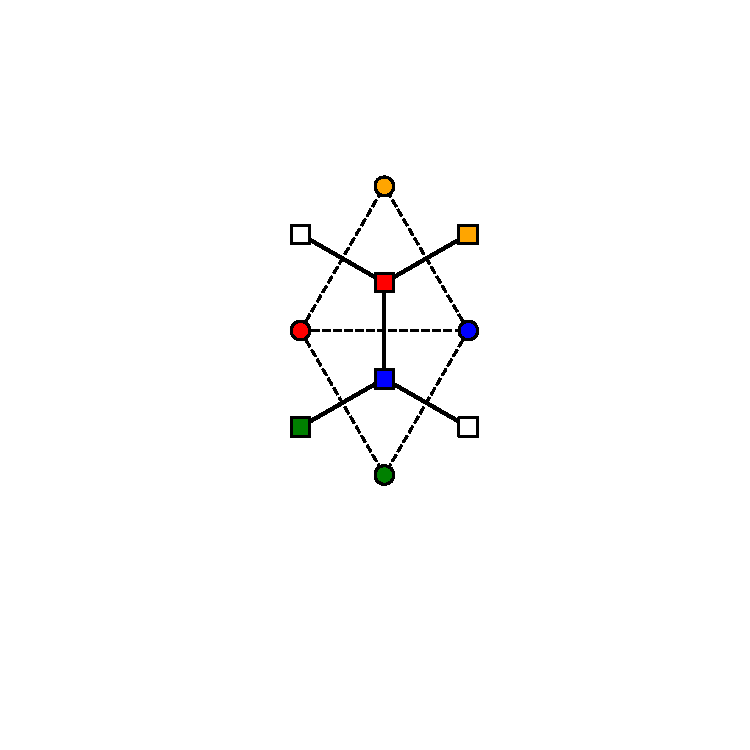
\includegraphics[height=2.6cm]{./figures/general_networks/bs_move_a.pdf}
         \caption{Initial $c=3$.}
         \label{fig:bsmovea}
     \end{subfigure}
     %{\LARGE$\rightarrow$}
     \hfill
     \begin{subfigure}[b]{0.25\textwidth}
         \centering
         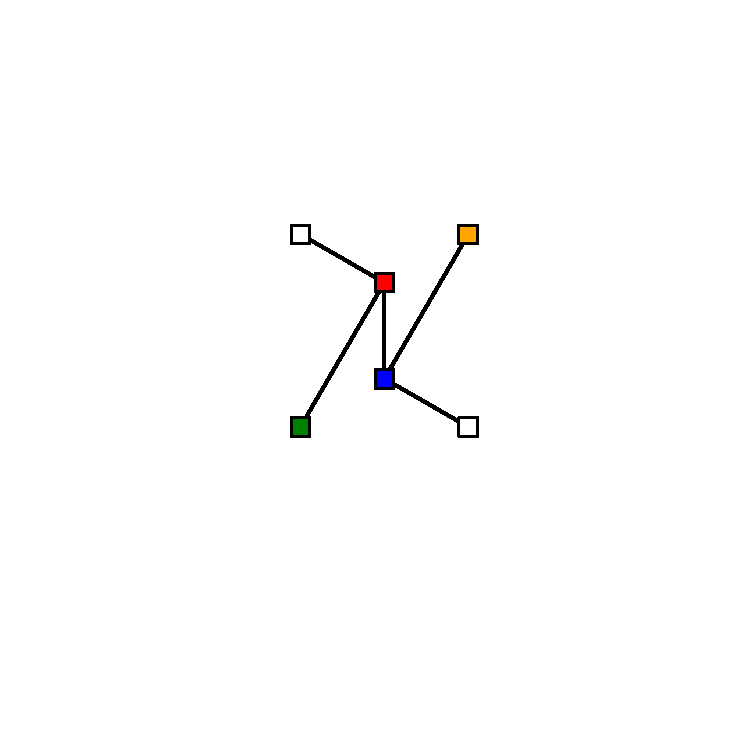
\includegraphics[height=1.8cm]{./figures/general_networks/bs_move_b.pdf}
         \caption{Switched $c=3$.}
         \label{fig:bsmoveb}
     \end{subfigure}
     %{\LARGE$\rightarrow$}
     \hfill
     \begin{subfigure}[b]{0.25\textwidth}
         \centering
         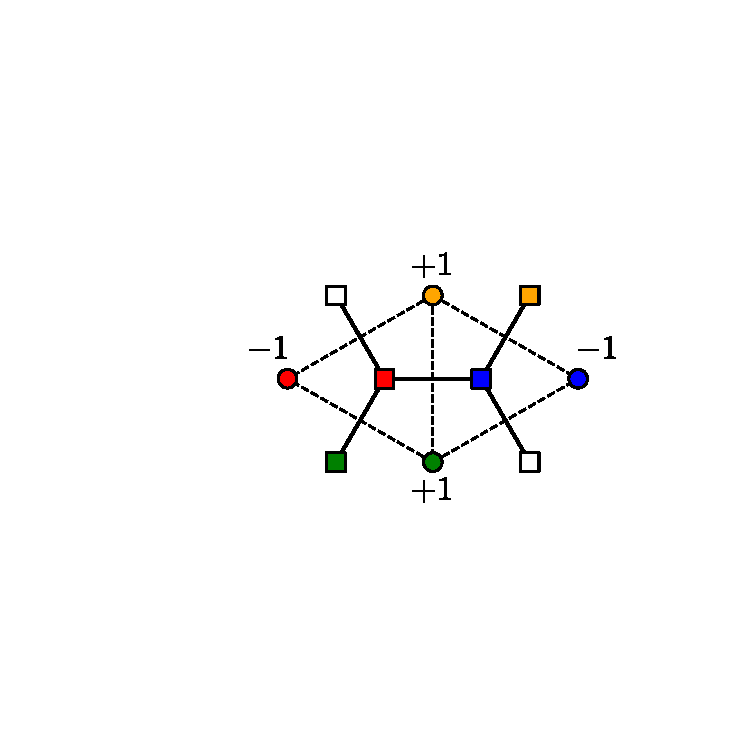
\includegraphics[height=2.1cm]{./figures/general_networks/bs_move_c.pdf}
         \caption{Optimised $c=3$.}
         \label{fig:bsmovec}
     \end{subfigure}
     
     \vspace{5mm}
     \begin{subfigure}[b]{0.25\textwidth}
         \centering
         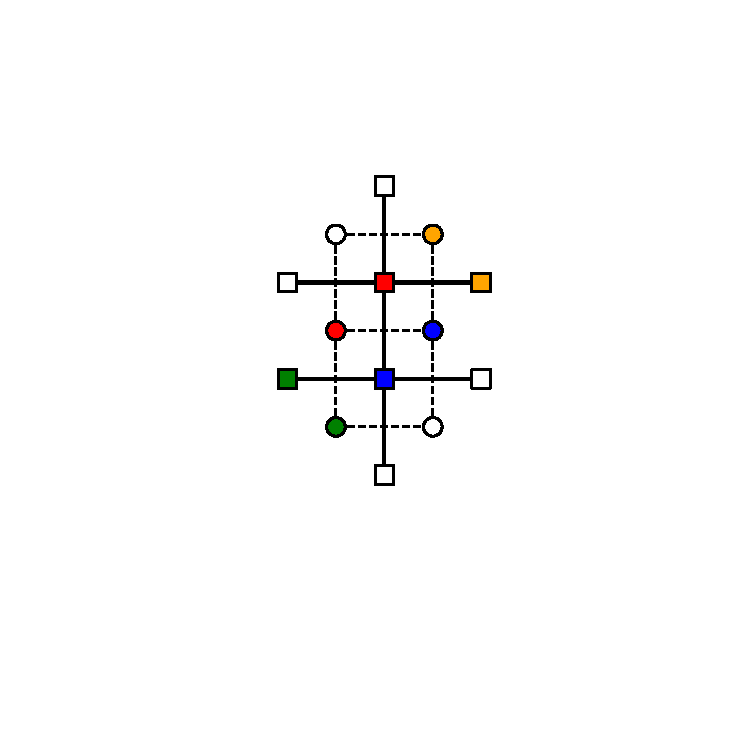
\includegraphics[height=2.6cm]{./figures/general_networks/bs_move_d.pdf}
         \caption{Initial $c=4$.}
         \label{fig:bsmoved}
     \end{subfigure}
     %{\LARGE$\rightarrow$}
     \hfill
     \begin{subfigure}[b]{0.25\textwidth}
         \centering
         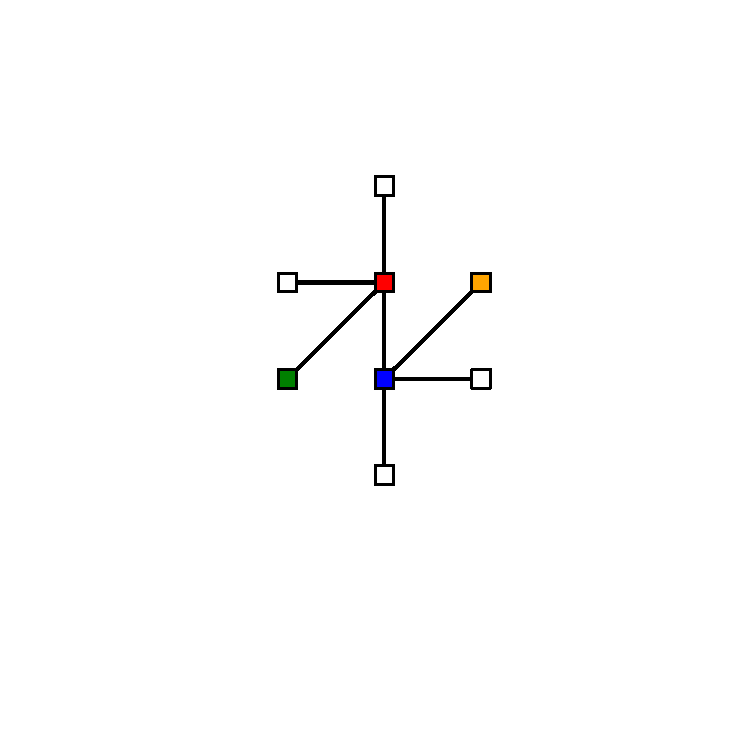
\includegraphics[height=2.6cm]{./figures/general_networks/bs_move_e.pdf}
         \caption{Switched $c=4$.}
         \label{fig:bsmovee}
     \end{subfigure}
     %{\LARGE$\rightarrow$}
     \hfill
     \begin{subfigure}[b]{0.25\textwidth}
         \centering
         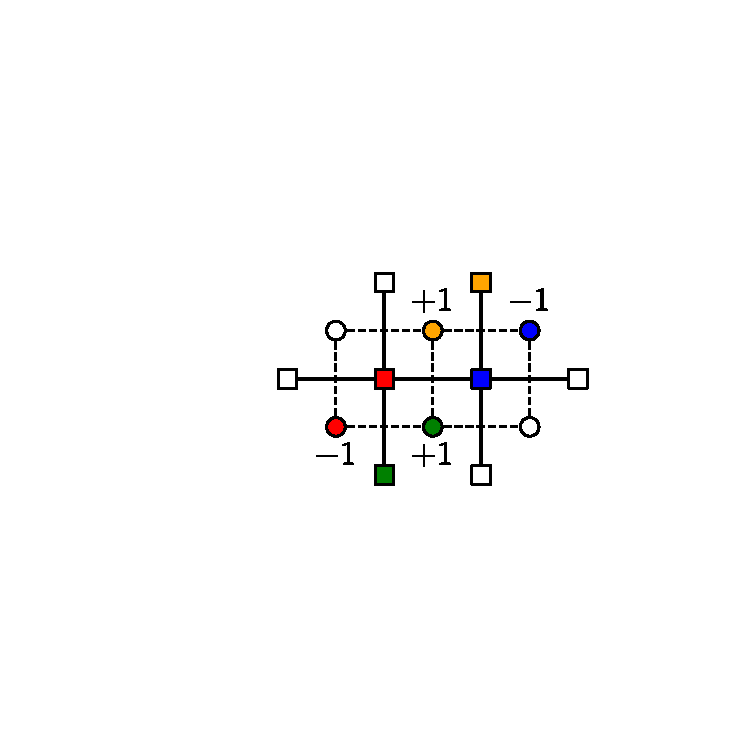
\includegraphics[height=1.8cm]{./figures/general_networks/bs_move_f.pdf}
         \caption{Optimised $c=4$.}
         \label{fig:bsmovef}
     \end{subfigure}
     
     \vspace{5mm}
     \begin{subfigure}[b]{0.25\textwidth}
         \centering
         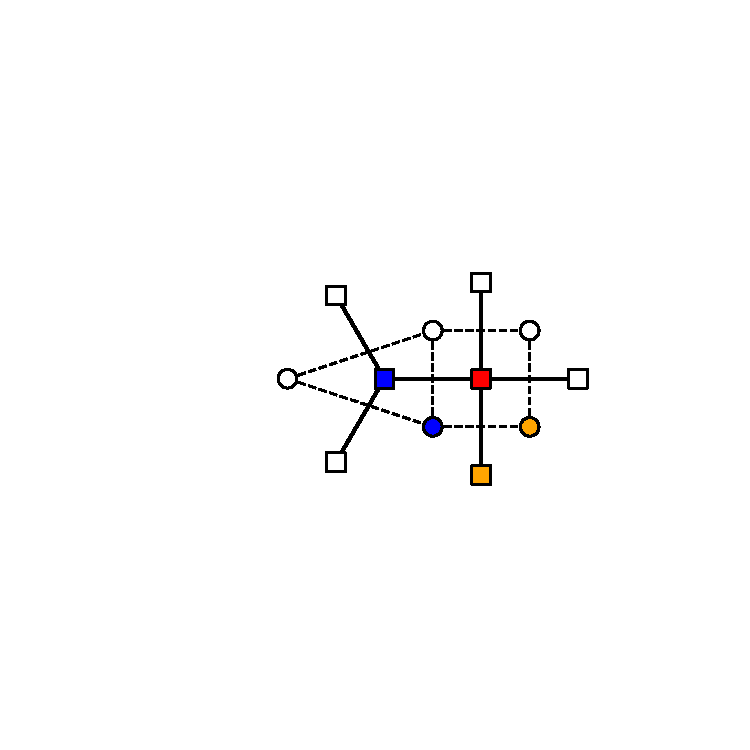
\includegraphics[height=1.8cm]{./figures/general_networks/bs_move_g.pdf}
         \caption{Initial $c=3,4$.}
         \label{fig:bsmoveg}
     \end{subfigure}
     %{\LARGE$\rightarrow$}
     \hfill
     \begin{subfigure}[b]{0.25\textwidth}
         \centering
         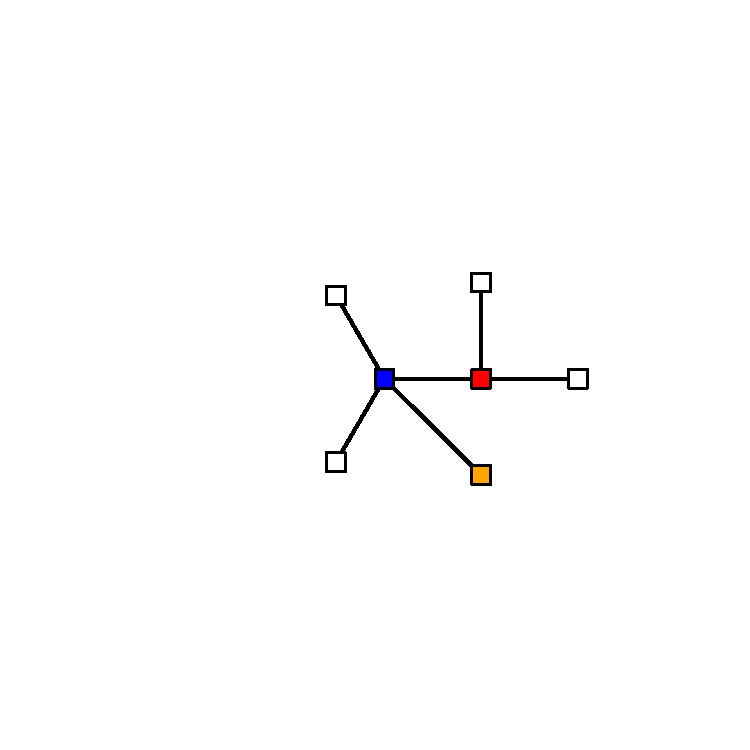
\includegraphics[height=1.8cm]{./figures/general_networks/bs_move_h.pdf}
         \caption{Switched $c=4,3$.}
         \label{fig:bsmoveh}
     \end{subfigure}
     %{\LARGE$\rightarrow$}
     \hfill
     \begin{subfigure}[b]{0.25\textwidth}
         \centering
         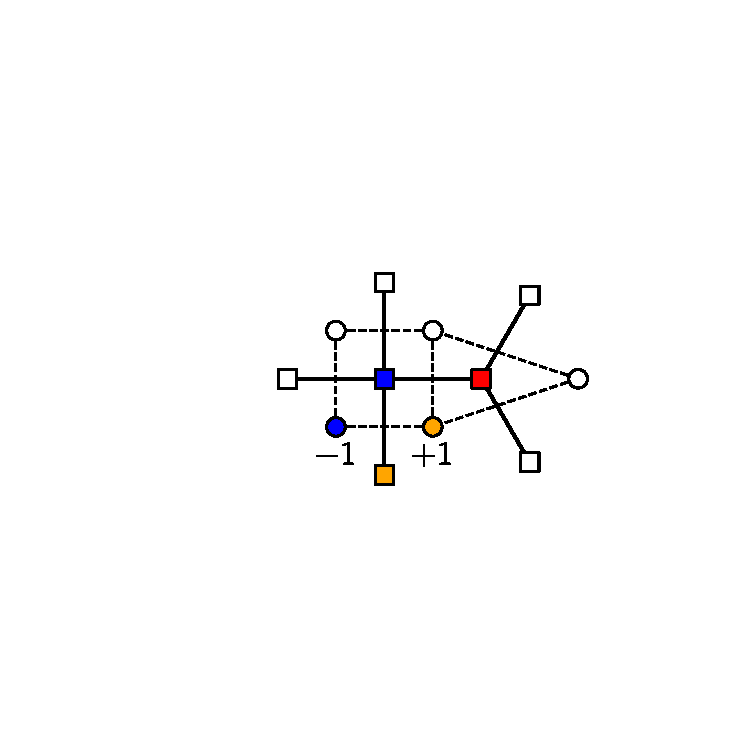
\includegraphics[height=1.8cm]{./figures/general_networks/bs_move_i.pdf}
         \caption{Optimised $c=4,3$.}
         \label{fig:bsmovei}
     \end{subfigure}
     
     \caption{Bond switching Monte Carlo moves for different atomic coordination environments: 3\--coordinate sites (a)-(c), 4\--coordinate sites (d)-(f) and mixed 3/4 coordination (g)-(i). For each coordination type the atomic connectivity is shown for the starting structure (left), the initial switched structure (middle), and a geometry optimised switched structure (right), via the squares and solid lines. The effect on the dual network (circles and dashed lines) is also demonstrated, with the numbers indicating the change in node degree after the move is applied. Colouring is used as a guide for the eye, to track changes between the pre\-- and post\--switch configurations.
}
     \label{fig:bsmoves}
\end{figure}

The thermalisation of the initial lattice requires a large number of random moves as described above, the purpose being for the system to ``forget'' all memory of the original ordered lattice. 
To ensure the lattice is fully randomised, observables such as the second moment of the ring sizes and assortativity can be monitored. For mixed lattices it is also important that the variously coordinated atoms are adjacent to the number of others as expected from pure chance, namely the binomial expansion of $\left(3x_3/\ki+4x_4/\ki\right)^2$.

A key aspect in the bond switching algorithm is the potential model, which is required for geometry optimisation after the transposition and evaluation of the system energy. 


The method naturally lends itself to the use of semi-empirical potentials which have explicit bonding and angular neighbour lists, and as such a popular choice is the Keating potential\cite{Keating1966,Barkema2000} or modifications thereof\cite{Jain2018}.
For this work we have used also opted to use a simplified two\--dimensional version of the Keating potential\cite{VonAlfthan2003} with the option of being augmented with a restricted bending (ReB) potential\cite{Bulacu2013}.
This has the form:
\begin{align}
        U = &\sum_{i,j \in \text{bonds}} \frac{k_r\left(r_{ij}-r_0\right)^2}{2} \\ \nonumber
         + &\sum_{i,j,k \in \text{angles}} \frac{k_\theta \left(\cos \theta_{ijk} - \cos \theta_0\right)^2}{f\left(\theta_{ijk}\right)},
\end{align}
where $r_0$ is the equilibrium separation between atoms and $\theta_0$ the equilibrium angle, and $k_r$, $k_\theta$ are the respective bond and angle force constants.
The equilibrium bond length was set equal for all interaction types and the equilibrium angles were set to $2\pi/c$ for $c$-coordinate atoms.
The function $f\left(\theta_{ijk}\right)$ can either be set to unity, or $f\left(\theta_{ijk}\right)=2\sin^2\theta_{ijk}$ to obtain the Simplified Keating (SK) and ReB potentials respectively.
In addition, to generate networks in spherical geometry, a simple harmonic restraining potential was added to all atoms to keep them on a sphere of a fixed radius.

The rational for choosing this potential is that we aim to obtain results for generic systems, generating configurations with a high-throughput approach.
This model captures the essential physics the problem, whilst remaining computationally tractable when producing a large number of samples.
The ratio of the force constants, $k_r/k_\theta$, can also be varied to transform the system from one which is more like atomic material (length dominated) to a foam (angle dominated).
In addition, the possibility of using the ReB angle potential is an elegant way to maintain ring convexity, providing that any non-convexity introduced by the bond switch is resolved before the geometry optimisation takes place.
Finally a major advantage of the bond switching algorithm is that a local geometry optimisation can be employed such that only the atoms in the immediate vicinity of the switching move need to be minimised to obtain an accurate structure\cite{Mousseau2001}, which in our work included all atoms within five coordination shells.

Unless otherwise stated, the results in this work were obtained for $1024$ ring systems for $\ki=3,4$, and $1152$ ring systems for $\ki=5$. Each was thermalised with $2\times 10^5$ random moves, and annealed over a further $4\times 10^6$  moves. For each system 100 simulations were run starting from different random seeds.




